\section{Data Exploration}
\label{section:Architecture:DataExploration}
In this section we will describe the main dataset given to us
by Prisguiden.no. The full Jupyter notebook exploration
is located at \cite{notebook-data-exploration}. This section will only
describe the highlights from that Notebook.

\subsection{Basic data structure}
As of \textit{23-11-2021} the dataset consists of 35966868 entries.
The oldest recorded data are from the beginning of 2019.
It consists of 9 features.
as shown in \autoref{table:features_market_insight_dataset}.
\begin{table}[htbp]
  \centering
  \caption{Features of the Market insight dataset}
  \label{table:features_market_insight_dataset}
  \begin{tabular}{|c|l|c|l|}\hline\hline
    Nr & Name            & Type             & Description                                 \\ \hline
    1  & id              & (int64)          & Unique identifier                           \\ \hline
    2  & product id      & (int64)          & Associated Product id                       \\ \hline
    3  & manufacturer id & (int64)          & Manufacturer id                             \\ \hline
    4  & cat id          & (int64)          & Associated category id                      \\ \hline
    5  & root cat id     & (int64)          & Associated root category id                 \\ \hline
    6  & date            & (datetime64[ns]) & The date the data was captured              \\ \hline
    7  & hits            & (int64)          & How many times the product page was visited \\ \hline
    8  & clicks          & (int64)          & How many times users clicked to a retailer  \\ \hline
    9  & last modified   & (object)         & When the row was last modified              \\ \hline
  \end{tabular}
\end{table}

It is worth noticing that hits and clicks are different features that measure the same thing: user interest.
A hit is how many times the product page on Prisguiden.no is visited.
A click is how many times a user follows a link from Prisguiden.no to an external retailer for a given product.
A product can receive a hit and not a click if the user just visits a product detail page without clicking to a retailer.
A product may receive a click without a hit if the user clicks on an AD or a campaign, which will lead the user directly to the retailer,
skipping the product page on Prisguiden.no.
The correlation between hits and clicks for all categories is roughly $0.578$.

The dataset consists of 1325 unique categories and 310499 unique products.
Each product is associated with a product category; for example,
all CPUs are associated with the category
\textit{"Prosessor (CPU)"s}.
Each product category is a leaf node of a category hierarchy.
The category \textit{"Prosessor (CPU)"} is a child of the parent category
\textit{"Datakomponenter"}, which itself is a child of \textit{"Data"}.

% Prisguiden.no are not interested in insight on the product level, but on the product category level.
Summing togheter all product clicks and hits to its closest parent category
gives us a table on the format shown in \autoref{table:market_insights_overview_11-12-21}.

\todo[inline]{Update table when we get new data from Prisguiden}
\import{./tables/code_generated/data_exploration/}{market_insights_overview_11-12-21.tex}

\subsection{Category plot analysis}
\autoref{fig:lineplot1} and \autoref{fig:lineplot2} show hits and clicks
from a random sample of categories from 2019 to 2021.
Most of the plots show a clear yearly periodic pattern, as shown in
\autoref{fig:lineplot-Hodetelefoner},
\autoref{fig:lineplot-Mobiltelefon},
\autoref{fig:lineplot-Julekalender}.
The scale of values differs between categories.
While \textit{"Varmepumpe"} \autoref{fig:lineplot-Varmepumpe} hower around 1000 hits per day,
the category \textit{"Mobiltelefon"} \autoref{fig:lineplot-Mobiltelefon} gets around 7500 hits per day.
Meanwhile, the values within each category can differ vastly.
\textit{"Spillkonsoller"} \autoref{fig:lineplot-Spillkonsoller} has a hit peak around 60000,
while it usually gets around 5000 hits per day.

Some categories experience extreme variations in traffic at different intervals.
One example of this is the category \textit{"Grafikkort GPU"}.
The traffic tracked before and after Christmas 2020 differs vastly,
and the data changes its behavior and distribution from then on.

\autoref{table:Mobiltelefon_statistics} shows some basic statistics for \textit{Mobiltelefoner}.
This exact category was chosen at random just to get an idea of how one-time series might behave.
The time series has a mean of 6453 hits and a standard deviation of 1881, which is
around 30\% of the mean. This is quite a big variance in the dataset.

% Mobiltelefon stats table
\import{./tables/code_generated/data_exploration/}{Mobiltelefon_statistics.tex}

It is interesting to see how many categories receive zero values and undefined values each day.
A zero value count in this context means how many days a given category has gotten 0 hits, but it has gotten some clicks.
A NaN value in this context means that the given category has gotten 0 clicks and 0 hits on the given day.
\autoref{fig:category_0_and_NaN_values} shows a lineplot of the different distributions.
In general, relatively few categories have 0-values.
Some of the first categories created, the ones with id 0-500, there exists some days with 0 interest.
However, most categories have at least one click and one hit each day.
Categories with id above 10000 start to see a lot more zero values.
The most likely explanation for this is that these categories are created at a later point in time.
The steadily growing line at the end of \autoref{fig:category_NaN_values} near id 12000 supports this theory.
\begin{figure}[h!]
  \centering
  \caption{Counting how many categories have days with 0 hits or NaN values}
  \label{fig:category_0_and_NaN_values}
  \begin{subfigure}[b]{0.4\textwidth}
    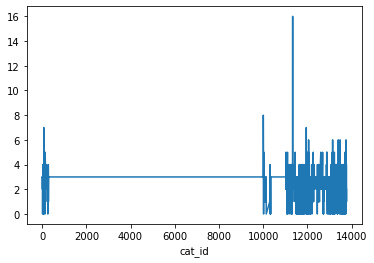
\includegraphics[width=\textwidth]{./figs/code_generated/data_exploration/category_0_values.png}
    \hfill
    \caption{0-values}
    \label{fig:category_0_values}
  \end{subfigure}
  \begin{subfigure}[b]{0.4\textwidth}
    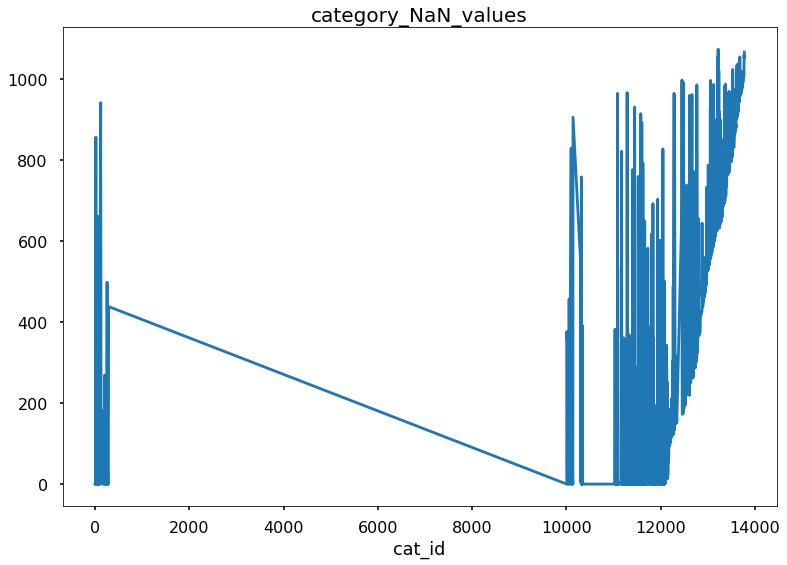
\includegraphics[width=\textwidth]{./figs/code_generated/data_exploration/category_NaN_values.png}
    \hfill
    \caption{NaN-values}
    \label{fig:category_NaN_values}
  \end{subfigure}
\end{figure}



\begin{figure}[h!]
  \centering
  \caption{Category plots of hits and click rate from 2019-2021}
  \label{fig:lineplot1}
  \begin{subfigure}[b]{\textwidth}
    \includegraphics[width=\textwidth]{./figs/code_generated/data_exploration/lineplot_51_Hodetelefoner og ørepropper.png}
    \hfill
    \caption{Hits and clicks rate for \textit{Hodetelefoner og ørepropper}}
    \label{fig:lineplot-Hodetelefoner}
  \end{subfigure}

  \begin{subfigure}[b]{\textwidth}
    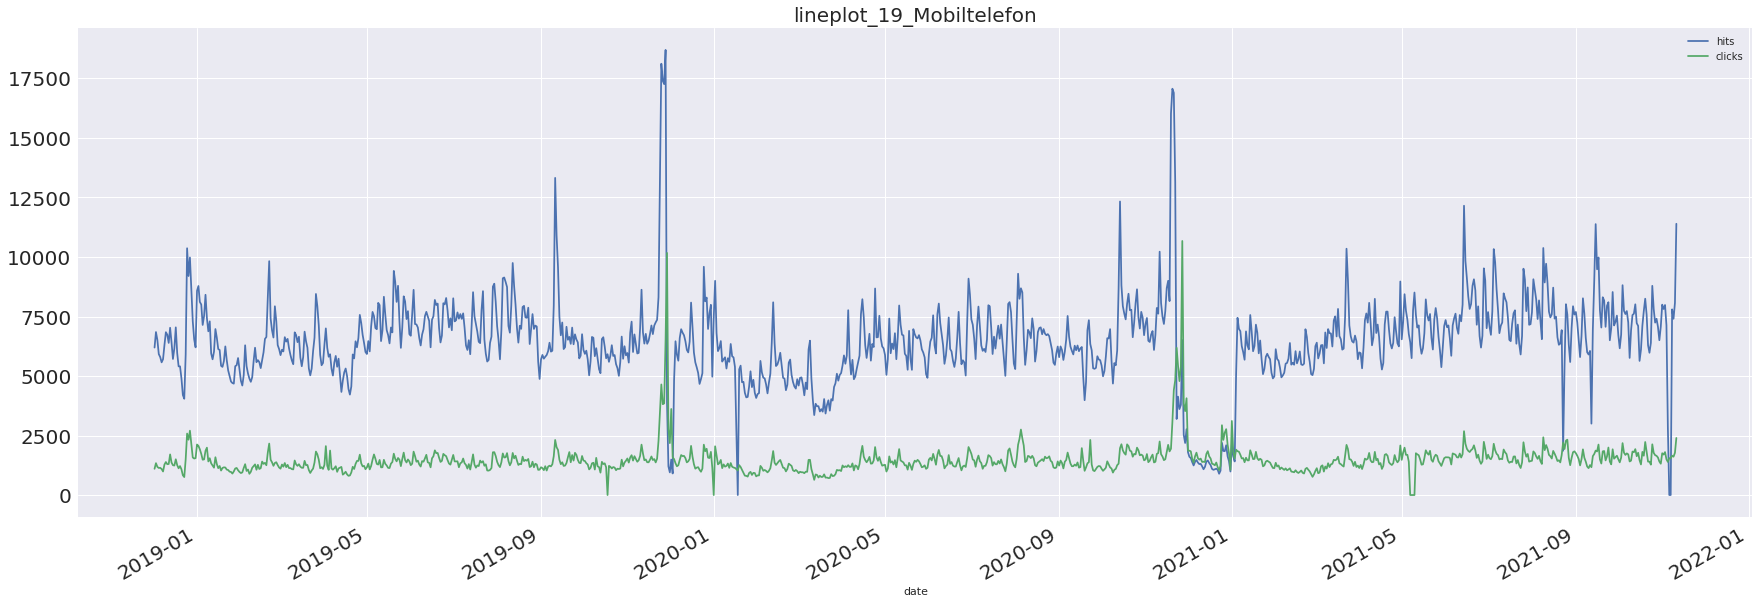
\includegraphics[width=\textwidth]{./figs/code_generated/data_exploration/lineplot_19_Mobiltelefon.png}
    \hfill
    \caption{Hits and clicks rate for \textit{Mobiltelefon}}
    \label{fig:lineplot-Mobiltelefon}
  \end{subfigure}

  \begin{subfigure}[b]{\textwidth}
    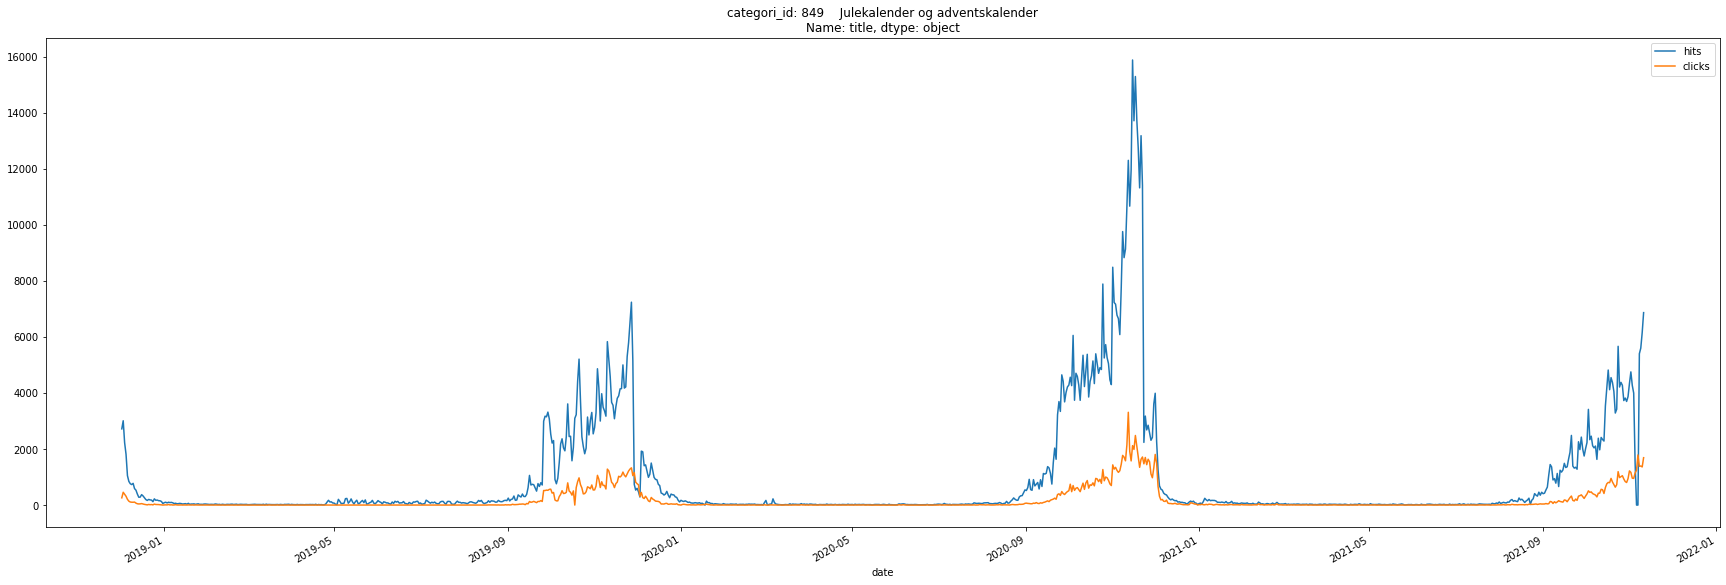
\includegraphics[width=\textwidth]{./figs/code_generated/data_exploration/lineplot_11781_Julekalender og adventskalender.png}
    \hfill
    \caption{Hits and clicks rate for \textit{Julekalender}}
    \label{fig:lineplot-Julekalender}
  \end{subfigure}
\end{figure}

\begin{figure}[h!]
  \centering
  \caption{Category plots of hits and click rate from 2019-2021}
  \label{fig:lineplot2}

  \begin{subfigure}[b]{\textwidth}
    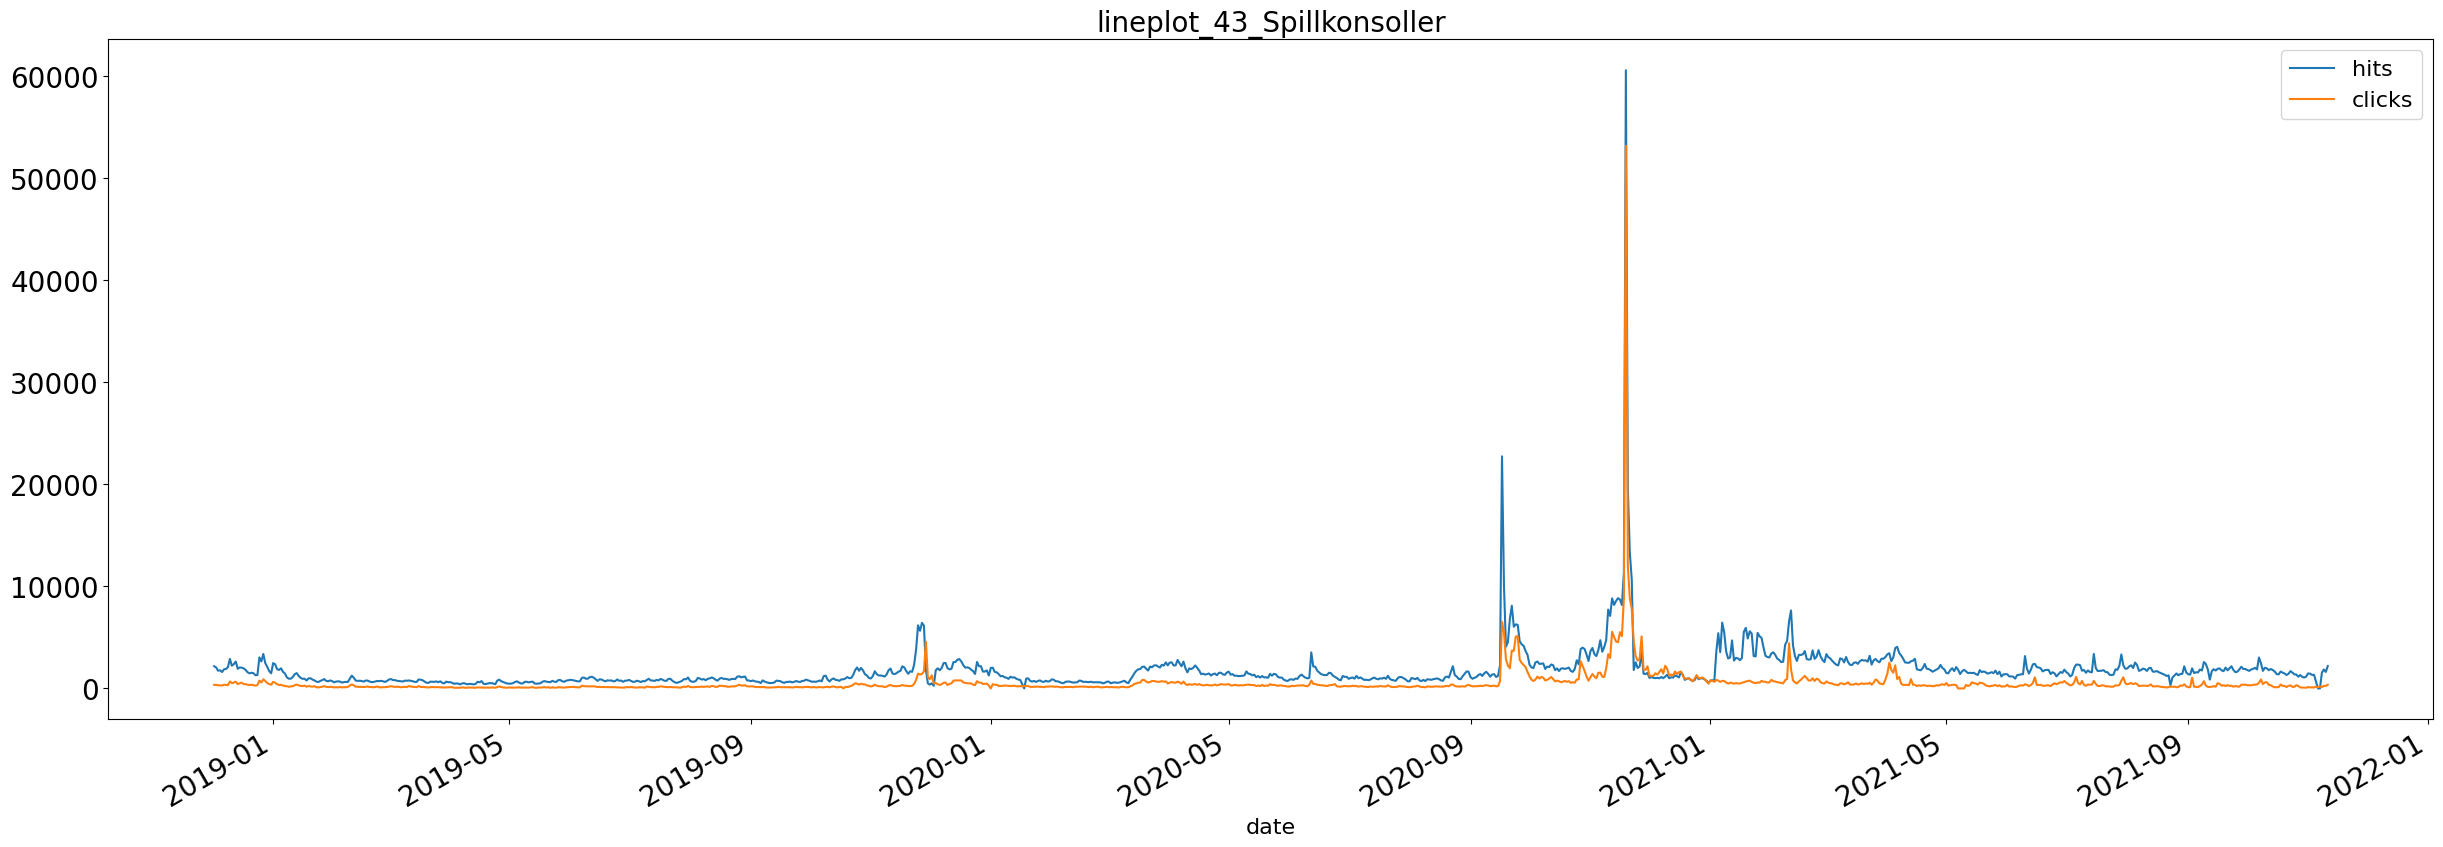
\includegraphics[width=\textwidth]{./figs/code_generated/data_exploration/lineplot_43_Spillkonsoller.png}
    \hfill
    \caption{Hits and clicks rate for \textit{Spillkonsoller}}
    \label{fig:lineplot-Spillkonsoller}
  \end{subfigure}
  \begin{subfigure}[b]{\textwidth}
    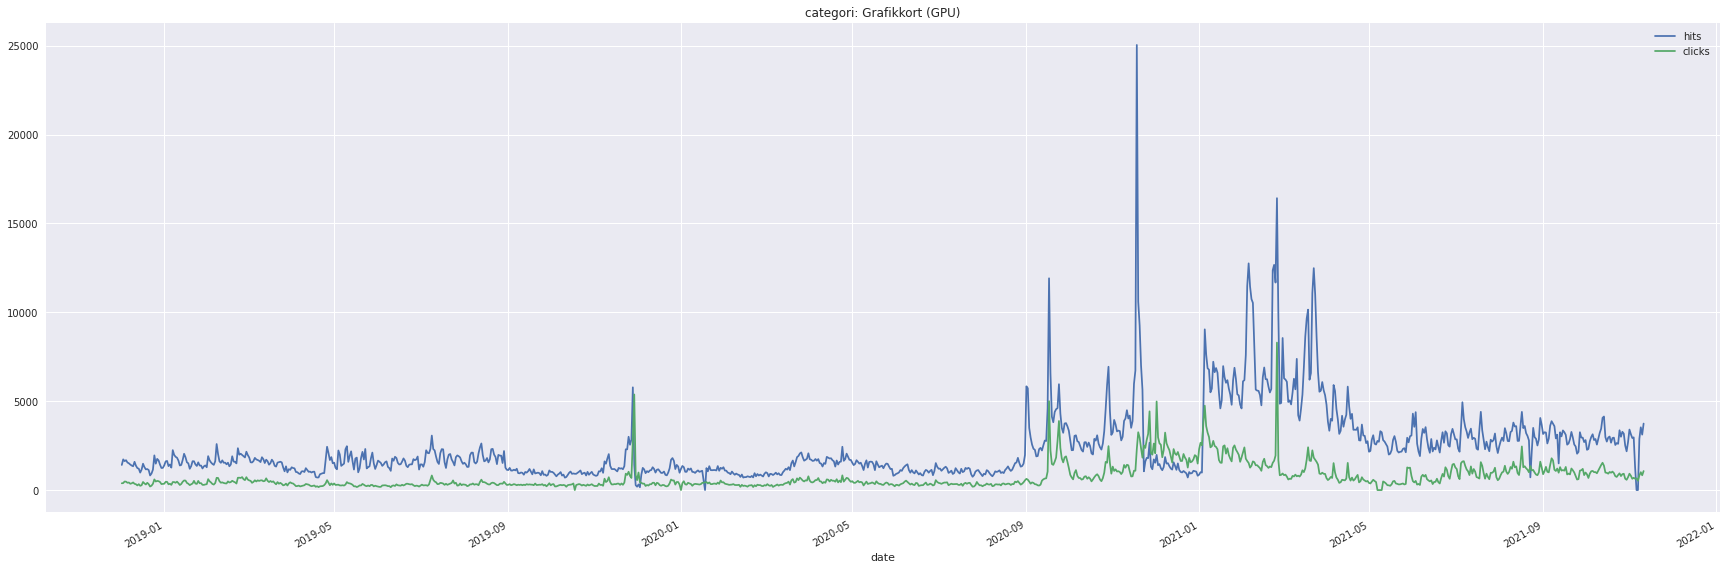
\includegraphics[width=\textwidth]{./figs/code_generated/data_exploration/lineplot_30_gpu.png}
    \hfill
    \caption{Hits and clicks rate for \textit{Grafikkort GPU}}
    \label{fig:lineplot-GPU}
  \end{subfigure}

  \begin{subfigure}[b]{\textwidth}
    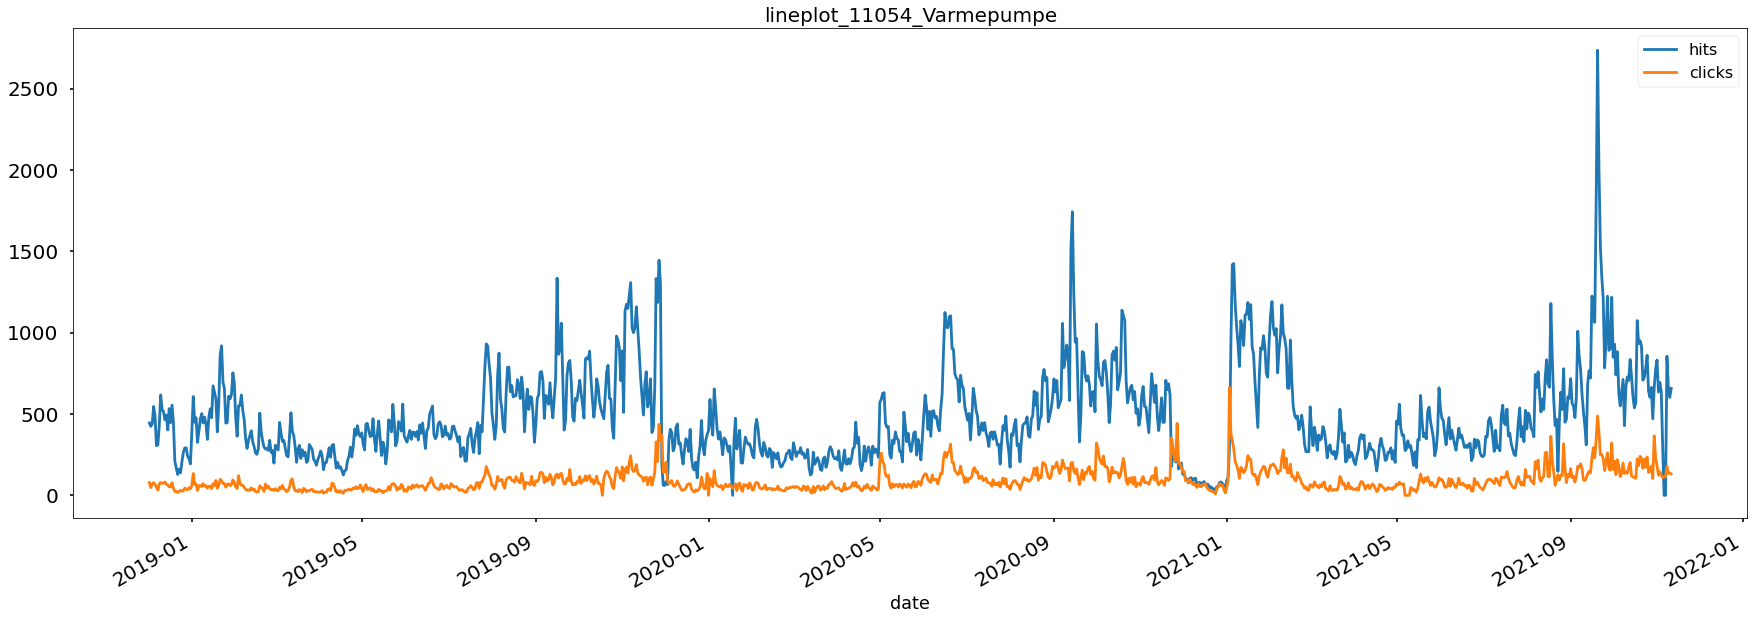
\includegraphics[width=\textwidth]{./figs/code_generated/data_exploration/lineplot_11054_Varmepumpe.png}
    \hfill
    \caption{Hits and clicks rate for \textit{Varmepumpe}}
    \label{fig:lineplot-Varmepumpe}
  \end{subfigure}
\end{figure}

\subsection{Correlation among categories}
Through a correlation analysis of the data, a correlation matrix is created.
Analyzing all categories with more than 100 datapoints, the values are compared and used to create the correlation matrix.
The matrix is shown in \autoref{fig:category_corelation_matrix}.
The lighter areas of the matrix indicate a correlation towards 1.0, while the darker areas indicate a correlation towards -1.0.

Based on the matrix's color spectrum, it is clear that categories cover almost the whole spectrum of correlation relationships.
The overall bright colors indicate a bias towards positive correlation.

\begin{figure}[h!]
  \centering
  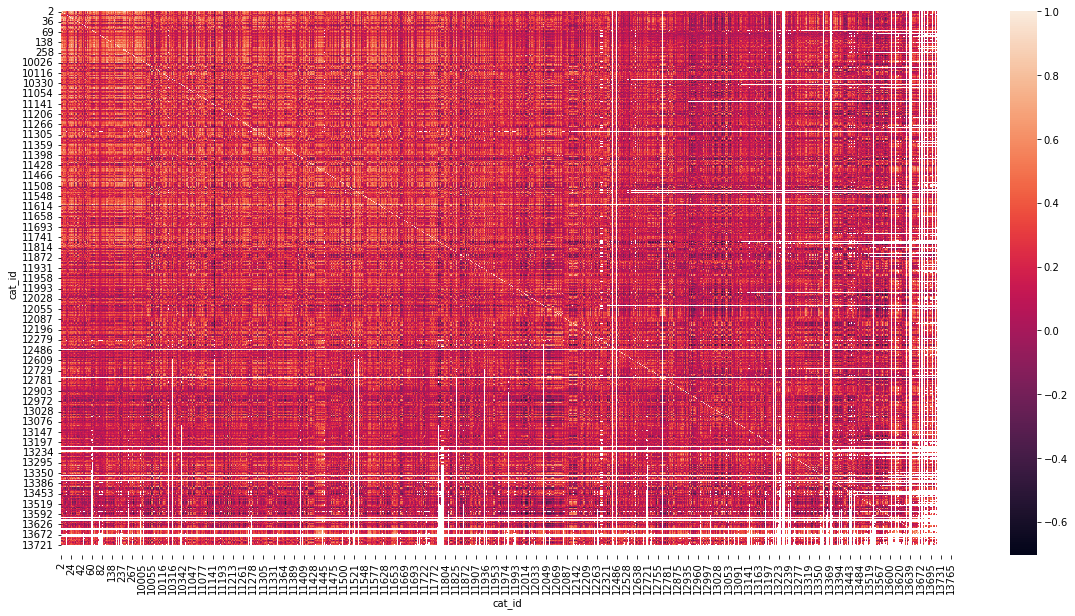
\includegraphics[width=\textwidth]{./figs/code_generated/data_exploration/category_correlation_matrix.png}
  \hfill
  \caption{Category correlation matrix}
  \label{fig:category_corelation_matrix}
\end{figure}





